\documentclass[12pt]{IEEEtran}
\usepackage[utf8]{inputenc}
\usepackage{cite}
\usepackage[hidelinks]{hyperref}
\usepackage{graphicx}
\usepackage{amsfonts}
\usepackage{mathtools}
\usepackage{caption}
\usepackage{fancyhdr}
\usepackage[ruled,vlined]{algorithm2e}
\usepackage{float}
\usepackage{listings}
\lstset{
basicstyle=\small\ttfamily,
columns=flexible,
breaklines=true
}

\pagestyle{fancy}
\fancyhf{}
\rhead{Search Engine Analysis}
\lhead{\thesection}
\rfoot{\thepage}

\DeclarePairedDelimiter\ceil{\lceil}{\rceil}
\DeclarePairedDelimiter\floor{\lfloor}{\rfloor}

\title{\textbf{Search Engine Analysis}\\Team \#2 - Semester}
\date{}

\begin{document}

% \thispagestyle{empty}

\maketitle

\begin{abstract}
  This document shows our analysis of the performance of our Search Engine and how we performed them.
\end{abstract}

\section{The Experiment}
\subsection{Running One Experiment}
This command runs the whole server in analysis mode and closes it after finishing the experiment. 

~\texttt{\$ env PAM=1 mvn}

\subsection{PerfAnalyser}
\texttt{PerfAnalyser.java} is the java class responsible for conducting one experiment and closing the server afterward. 
It does the following:
\begin{enumerate}
  \item Launches \small\texttt{\$TOTAL\_THREADS} of threads, each calls \small\texttt{Query Processor} with a random query.
  \item After timeout of \small\texttt{\$TIMEOUT\_MS}, \small\texttt{PerfAnalyser.java} interrupts threads that didn't finish, then collects the time of the rest of the threads.
  \item Calculates the average time of all threads, and calculates the number of timeouted threads.
  \item Repeats this experiment one time again with the ranker disabled.
  \item Queries the size of all crawled documents and the number of indexed keywords.
  \item Serializes all the collected data into json file whose name follows the pattern \small\{\texttt{performance-analysis-\$\{TIME\}.json}\} and saves it into current working directory.
\end{enumerate}

\subsection{Repeating}
You need to conduct this experiment multiple times during different stages of search engine running. Then plot the results to be able to answer the performance questions.

To plot the results with the python script:
\begin{lstlisting}
  $ python3 plot.py $PWD perf*.json
\end{lstlisting}

\section{Results}
Setting \small\texttt{\$TOTAL\_THREADS} = 200, \small\texttt{\$TIMEOUT\_MS} = 2 Minutes and running \small\texttt{PerfAnalyser.java} 10 times at different stages of database building.
We got 2 figures, Fig. \ref{fig:avgtime}, and a flat line at $1$ for the 'Success Precentage vs. Crawled Pages and Indexed keywords.'

\begin{figure}
  \centering
  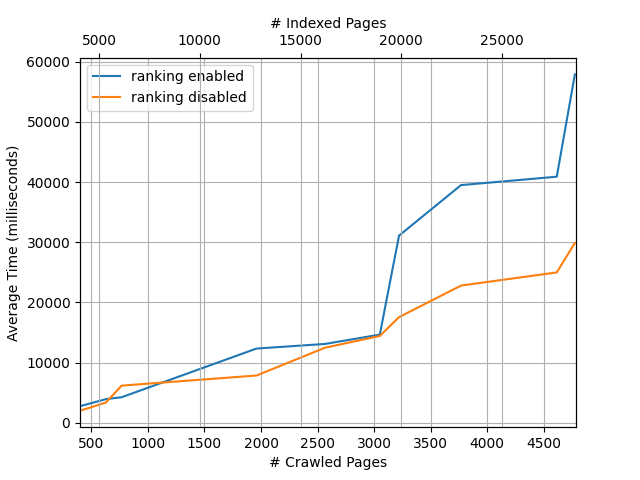
\includegraphics[width=\linewidth]{avgtime.png}
  \caption{Average Time vs. Num. Crawled Pages and Indexed keywords}
  \label{fig:avgtime}
\end{figure}

% \begin{figure}
%   \centering
%   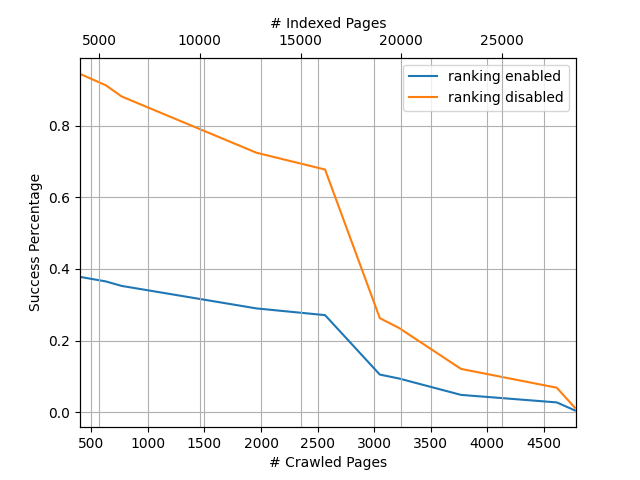
\includegraphics[width=\linewidth]{secPrec.png}
%   \caption{Success Percentage vs. Num. Crawled Pages and Indexed keywords}
%   \label{fig:secPrec}
% \end{figure}

\section{Discussion}
After experimenting with query processor through a range of crawled pages up to $4000$ and indexed words up to $80000+$, we notice that the speed of query processor both with and without ranking is affected by the database size. However, the success rate is always one, as the query processor never fails with up to $200$ simultaneous requests. This is due to the following:
\begin{itemize}
    \item In our implementation, There are multiple threads that run in parallel for crawler, indexer, popularity ranker and query processor. This results in a huge amount of database queries from all parallel threads. Consequently, by increasing the size of database, the size of query results increases, which, in return, increases the number of database access in both query processor and ranker slowing down the query response.
    \item We use \emph{CoreNLP} library in the query processor, which consumes a lot of time performing \texttt{NER} \emph{(Named-Entity Recognition)} on each query string.
\end{itemize}

\section{Conclusion}
In conclusion, we can state that the main downsides about the performance of our implementation are \emph{excess number of database access from all components at the same time} and \emph{the usage of external libraries for some specialized tasks.}

\end{document}